\documentclass{article}

\usepackage{amsmath, mathtools, amsthm}

\usepackage{graphicx}
\graphicspath{ {./images/automi} }

\title{Automi}
\author{github.com/asdrubalini}
\date{\today}

\begin{document}
    \maketitle

    Automa: software generico che può funzionare su qualsiasi dispositivo programmabile.
    Un automa può essere progettato graficamente con l'utilizzo di due simboli: freccia e cerchio.
    Una volta che la progettazione è conclusa, l'automa deve essere programmato con un vero e proprio linguaggio di programmazione.

    \begin{center}
        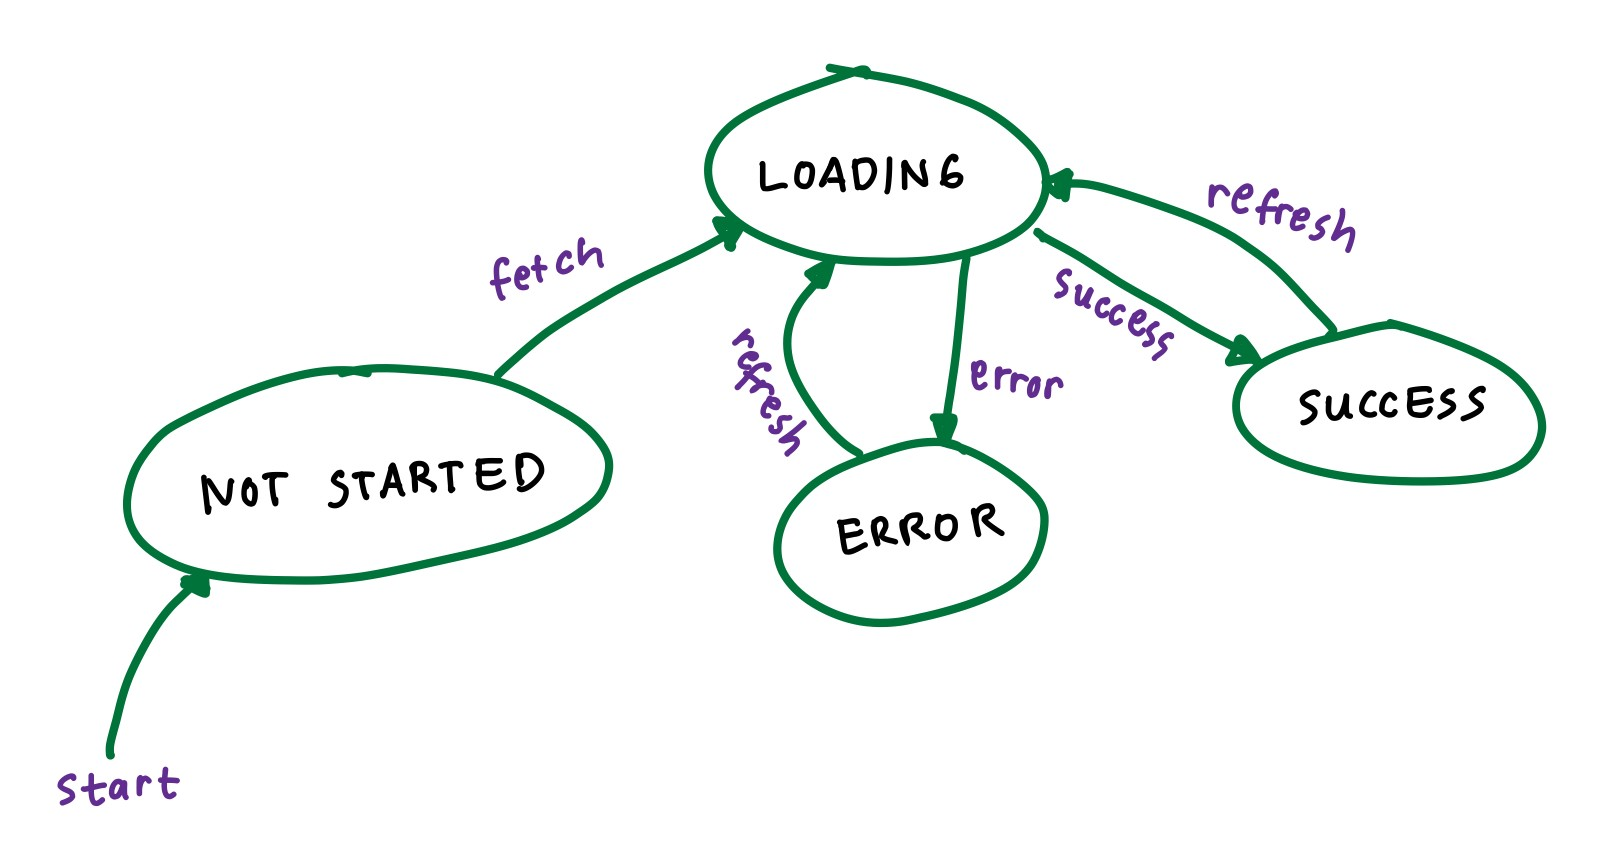
\includegraphics[width=\textwidth]{automa.png}
        Esempio di diagramma che descrive un'automa
    \end{center}

\end{document}
